% 依据固定来源 PDF 第 1 页的点位、棱线和虚实关系重绘；示意图不按比例
% source_id=src-3612a22ce3848ad6ebbec4d94861dd64b009980e14e8c7a83efefb2ea39bd367
% PDF SHA-256: 2cea664b02860c04aa21fb6bdf80403b674befb8e61fa9f68970197bdf0f5ff4
\begin{center}
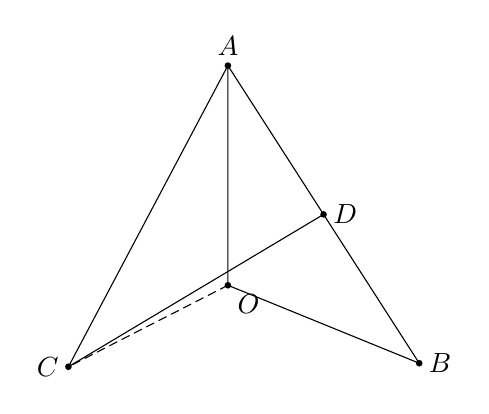
\begin{tikzpicture}[x=0.9cm,y=0.9cm,line join=round,line cap=round]
  \coordinate (A) at (0,3.1);
  \coordinate (O) at (0,0);
  \coordinate (B) at (2.7,-1.1);
  \coordinate (C) at (-2.25,-1.15);
  \coordinate (D) at (1.35,1.0);
  \draw (A)--(B)--(O)--cycle;
  \draw (A)--(C);
  \draw[densely dashed] (O)--(C);
  \draw (C)--(D);
  \fill (A) circle (1.2pt) node[above] {$A$};
  \fill (B) circle (1.2pt) node[right] {$B$};
  \fill (C) circle (1.2pt) node[left] {$C$};
  \fill (O) circle (1.2pt) node[below right] {$O$};
  \fill (D) circle (1.2pt) node[right] {$D$};
\end{tikzpicture}
\end{center}
